\documentclass[a4paper,12pt]{article}

\usepackage[utf8]{inputenc}
\usepackage{amsmath,amssymb,graphicx,natbib,float,xcolor,geometry,mathptmx}
\usepackage{wrapfig}
\usepackage{subfig}
\usepackage{lipsum}

%%%% ---- Formatting ---- %%%%

% margins
\geometry{a4paper, top=40mm, right=25.4mm, bottom = 25.4mm, left = 25.4mm}

% links
\usepackage[pdfusetitle]{hyperref}
\hypersetup{hidelinks,colorlinks,urlcolor=[rgb]{0,0,1}}

% paragraph formatting
\setlength{\parskip}{12pt plus 0.2ex minus 0.2ex}
\setlength{\parindent}{0pt}

% figure captions
\usepackage[font=small,labelfont=bf,margin=10pt]{caption}

% define keywords, title page and document properties
\makeatletter
  
  % define keywords variable
  \def\@keywords{}
  \newcommand{\keywords}[1]{
    \def\@keywords{#1}
  }

  % make title page
  \def\@maketitle{%
  \newpage
  \null
  {\centering
  \let \footnote \thanks
    {\Large \bfseries \@title \par}%
    \vskip -4pt%
    {\it \@author \par}%
  \par}
  \vskip 12pt
 	\underline{keywords}: \@keywords
  }

%  % add info to pdf metadata
%  \hypersetup{pdftitle={\@title},pdfauthor={\@author}}

\makeatother

% change section heading
\makeatletter
\renewcommand\section{\@startsection {section}{1}{\z@}%
                                   {36pt}%
                                   {0.5pt \@plus.5pt}%
                                   {\centering\normalfont\bfseries}}
\makeatother


% bibliography
\bibliographystyle{plainnat}
\setcitestyle{authoryear}



%%%% ---- Abstract Properties ---- %%%%

\title{Efficient Origami Construction of Orthogonal Terrains using Cross Section Evolution}

\author{C. J. H. Dickens, G. Orwell, G. R. R. Martin}
\keywords{cross sections, orthogonal terrains, time evolution}


%%%% ---- Start Document ---- %%%%

\begin{document}

\maketitle


\section*{Abstract}

We introduce a new method of origami construction, using cross section diagrams.
Instead of beginning our construction from a 2-dimensional sheet of paper,
we consider a 1-dimensional cross section moving forwards in time.

\graphicspath{{../figures/strip_narrowing/}}
\begin{wrapfigure}{r}{0.6\textwidth}
\vspace{-4.0em}
    \begingroup
    \def\svgwidth{0.19\textwidth}
        \captionsetup[subfigure]{width=0.17\textwidth}%
        \subfloat[Trivial cross section.] {
            \input{../figures/strip_narrowing/strip0.pdf_tex}%
        }%
    \endgroup%
    \begingroup
        \captionsetup[subfigure]{width=0.40\textwidth}%
        \def\svgwidth{0.19\textwidth}
        \subfloat[New zero length segment inserted at left endpoint. Existing segment reverses velocity.] {
            \input{../figures/strip_narrowing/strip11.pdf_tex}%
            \def\svgwidth{0.19\textwidth}
            \input{../figures/strip_narrowing/strip12.pdf_tex}%
        }%
    \endgroup%
    \vspace{-0.8em}
    \begingroup
    \def\svgwidth{0.19\textwidth}
        \captionsetup[subfigure]{width=0.38\textwidth}%
        \subfloat[New segment (red) inserted. Existing segments retain their velocities.] {
            \input{../figures/strip_narrowing/strip21.pdf_tex}%
            \def\svgwidth{0.19\textwidth}
            \input{../figures/strip_narrowing/strip23.pdf_tex}%
        }%
    \endgroup%
    \begingroup
    \def\svgwidth{0.19\textwidth}
        \captionsetup[subfigure]{width=0.19\textwidth}%
        \subfloat[Leftmost (blue) segment vanishes.] {
            \input{../figures/strip_narrowing/strip31.pdf_tex}%
        }%
    \endgroup%
    %\begingroup
    %\hspace{0.8em}
    %\def\svgwidth{0.42\textwidth}
        %\captionsetup[subfigure]{width=0.38\textwidth}
        %\subfloat[Side view of strip narrowing gadget, with layers separated.] {
        %\input{../figures/strip_narrowing/strip_layers.pdf_tex}
        %}%
    %\endgroup%
    \caption{Cross section evolution of a strip narrowing gadget. Segment velocities are denoted by (different colored) arrows.}
    \label{fig:strip_narrowing}
    \vspace{-1em}
\end{wrapfigure}
A cross section is a set of contiguous straight line segments
$$\mathcal C = \langle s_1, s_2,\cdots s_n \rangle$$
Each segment $s$ is associated with a velocity vector $\vec{\hat v_s}$.
The segments evolve according to their velocities, in a manner that preserves distances.
During this process, the segment lengths may change.

In a cross section, new segments may be inserted and zero length segments can be deleted at any time.
We may also alter the velocity of one or many segments at any time.
The area swept out by the cross section in the resulting evolution forms the folded state.
A basic example of cross section evolution for a \emph{strip narrowing gadget} is shown in Figure~\ref{fig:strip_narrowing}.

\begin{wrapfigure}{l}{0.3\textwidth}
    \vspace{-3.0em}
    \subfloat[Orthogonal terrain.] {
        \includegraphics[width=\linewidth]{../figures/terrain.png}
        \label{fig:terrain}
    }
    \vspace{-0.7em}
    \graphicspath{{../figures/}}
    \def\svgwidth{0.3\textwidth}
    \subfloat[Column extrusion.] {
        \input{../figures/column_extrusion.pdf_tex}%
        \label{fig:column_extrusion}
    }
    \vspace{-5.8em}
\end{wrapfigure}
We obtain conditions for the validity of a particular cross section evolution sequence,
and prove that the resulting folded state is \emph{isometric} to a flat sheet of paper.

Subsequently, we use this machinery to design an efficient construction of orthogonal terrains, with \emph{arbitrary rational extrusion heights}.
An orthogonal terrain is a $n\times m$ grid, along with a matrix $\left\{ E_{i,j}\right\}_{i\in [n], j\in[m]}$ of extrusion heights,
such that the face of the grid corresponding to the location $(i,j)$ coincides with the plane $z = E_{i,j}$ (Figure~\ref{fig:terrain}).

We begin by constructing a single column (Figure~\ref{fig:column_extrusion}) of the extrusion, by constructing level shift gadgets.
The cross section evolution of the level shift gadgets is shown in Figure~\ref{fig:level_shift_layers},~\ref{fig:level_shift}.

\graphicspath{{../figures/}}
\begin{wrapfigure}{l}{0.7\textwidth}
    \def\svgwidth{0.7\textwidth}
    \input{../figures/level_shift_layers.pdf_tex}%
    \caption{
    Cross section change from level $H_i$ to $H_{i+1}$. In reality, the blue segments is folded flat.
    The velocities of horizontal and vertical segments are shown by purple and green arrows respectively.
    }
    \label{fig:level_shift_layers}
\end{wrapfigure}
\begin{wrapfigure}{l}{0.7\textwidth}
    \graphicspath{{../figures/level_shift/}}
    \begingroup
        %\captionsetup[subfigure]{width=\textwidth}
        \def\svgwidth{0.14\textwidth}
        \subfloat {
            \input{../figures/level_shift/column1.pdf_tex}
        %}%
        \def\svgwidth{0.16\textwidth}
        \graphicspath{{../figures/level_shift/}}
        %\subfloat {
            \input{../figures/level_shift/column3.pdf_tex}%
        %}%
        \def\svgwidth{0.18\textwidth}
        \graphicspath{{../figures/level_shift/}}
        %\subfloat {
            \input{../figures/level_shift/column5.pdf_tex}%
        %}%
        \def\svgwidth{0.20\textwidth}
        \graphicspath{{../figures/level_shift/}}
        %\subfloat {
            \input{../figures/level_shift/column7.pdf_tex}%
        }%
    \endgroup%
    \caption{Level-shifting gadget.}
    \label{fig:level_shift}
\end{wrapfigure}
\graphicspath{{../figures/}}
\begin{wrapfigure}{r}{0.25\textwidth}
    \vspace{-25em}
    \def\svgwidth{0.25\textwidth}
    \input{../figures/boundaries.pdf_tex}%
    \caption{Boundaries of adjacent column extrusions. The zig-zag motion is shown in Figure~\ref{fig:level_shift}}
    \label{fig:boundaries}
    \vspace{-1.1em}
\end{wrapfigure}

Finally, we need to attach adjacent column extrusions together using a \emph{strip connector} gadget.
The boundaries of adjacent column extrusions are shown in Figure~\ref{fig:boundaries}.
We construct a connector gadget (Figure~\ref{fig:connector_gadget}) to fit the gap between the boundaries.
The final attachment of the connector and the column extrusion is shown in Figure~\ref{fig:column_connector}.

This completes the construction of the full orthogonal terrain Figure~\ref{fig:full_consruction}.
Assuming that the top faces of the terrain form axis aligned rectangles in the unfolded state,
we show that our construction can be made $2$-optimal in terms of paper usage.
\begin{figure}[!ht]
    \centering
    \subfloat[] {
        \includegraphics[width=0.5\textwidth]{../figures/full/full_unfold.png}%
        \label{fig:full_unfold}
    }%
    \subfloat[] {
        \includegraphics[width=0.5\textwidth]{../figures/full/full_fold.png}%
        \label{fig:full_fold}
    }%
    \graphicspath{{../figures/column_connector}}
    \subfloat[Connector] {
        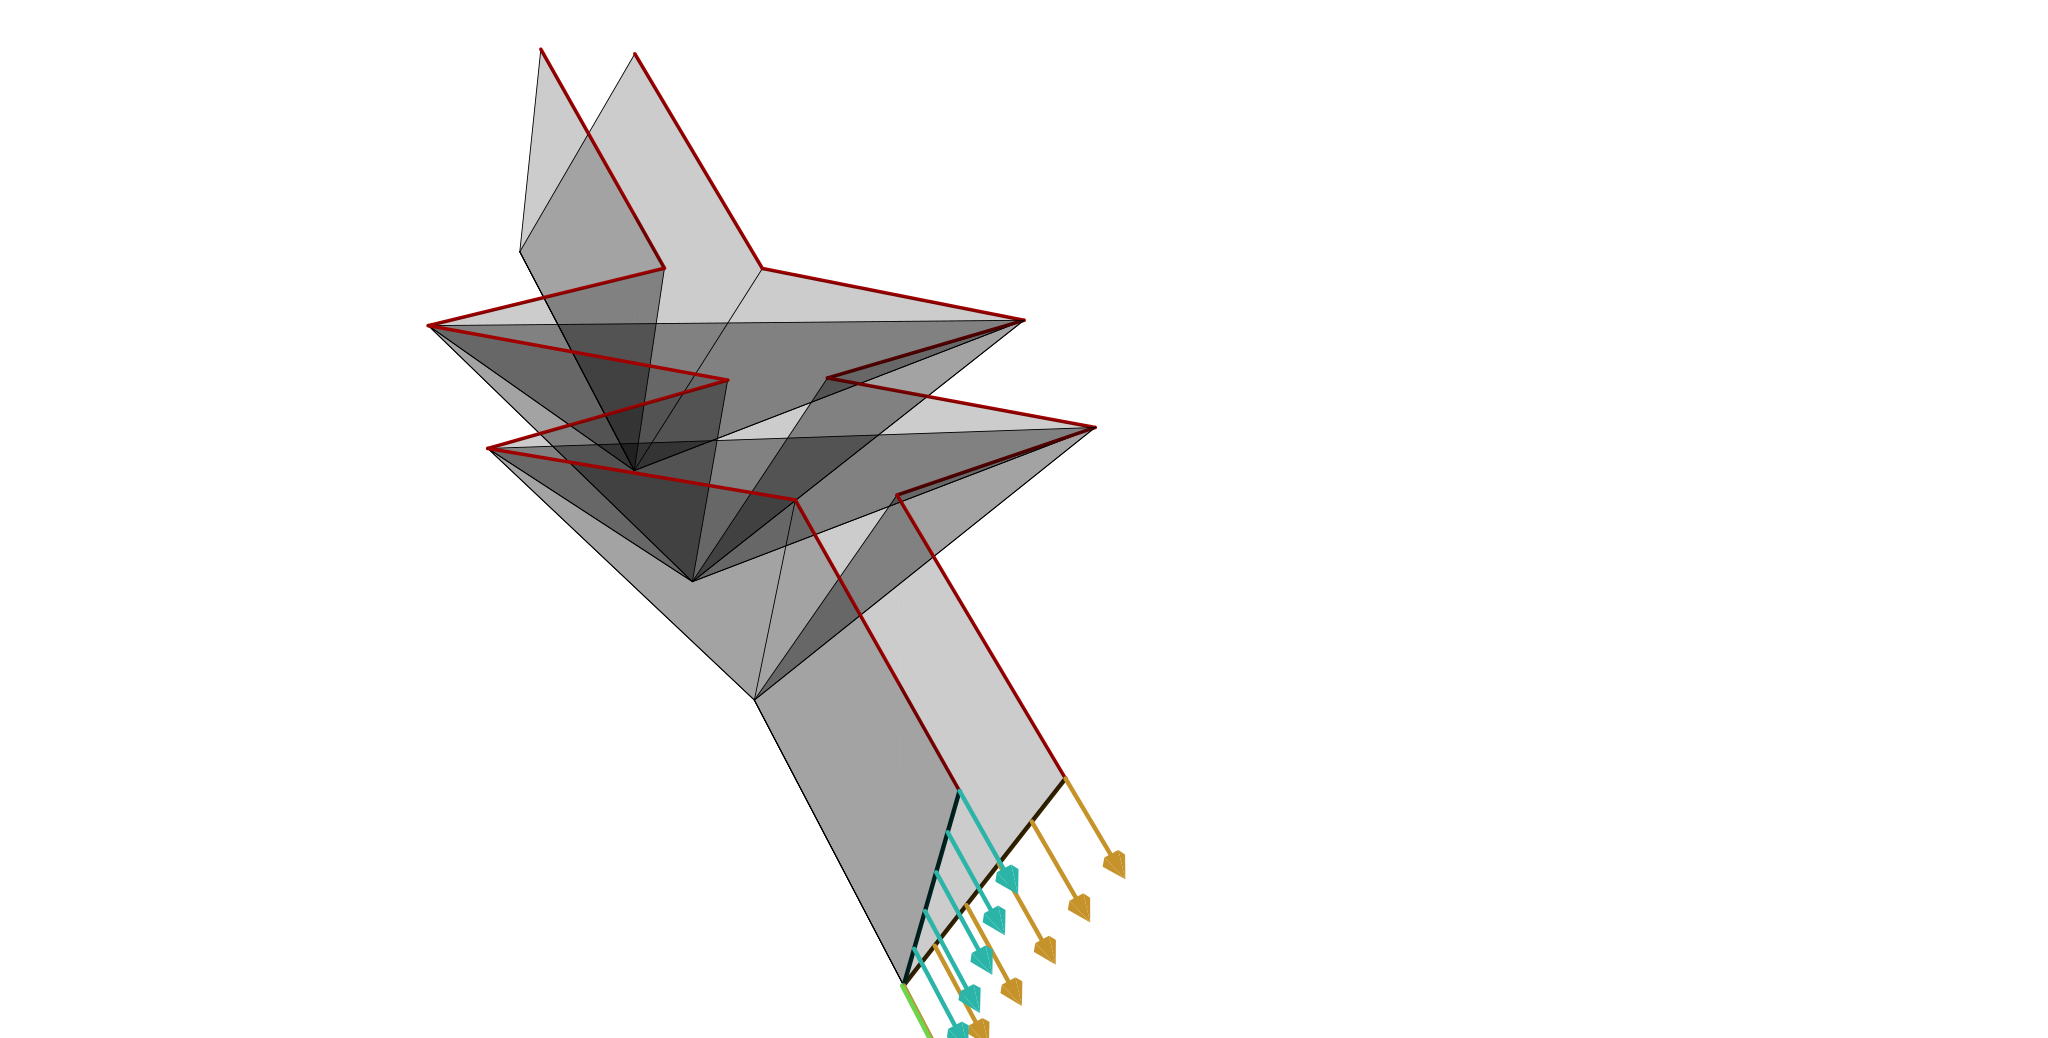
\includegraphics[width=0.2\textwidth]{../figures/column_connector/connector0.pdf}%
        \label{fig:connector_gadget}
    }%
    \subfloat[Connector with column.] {
        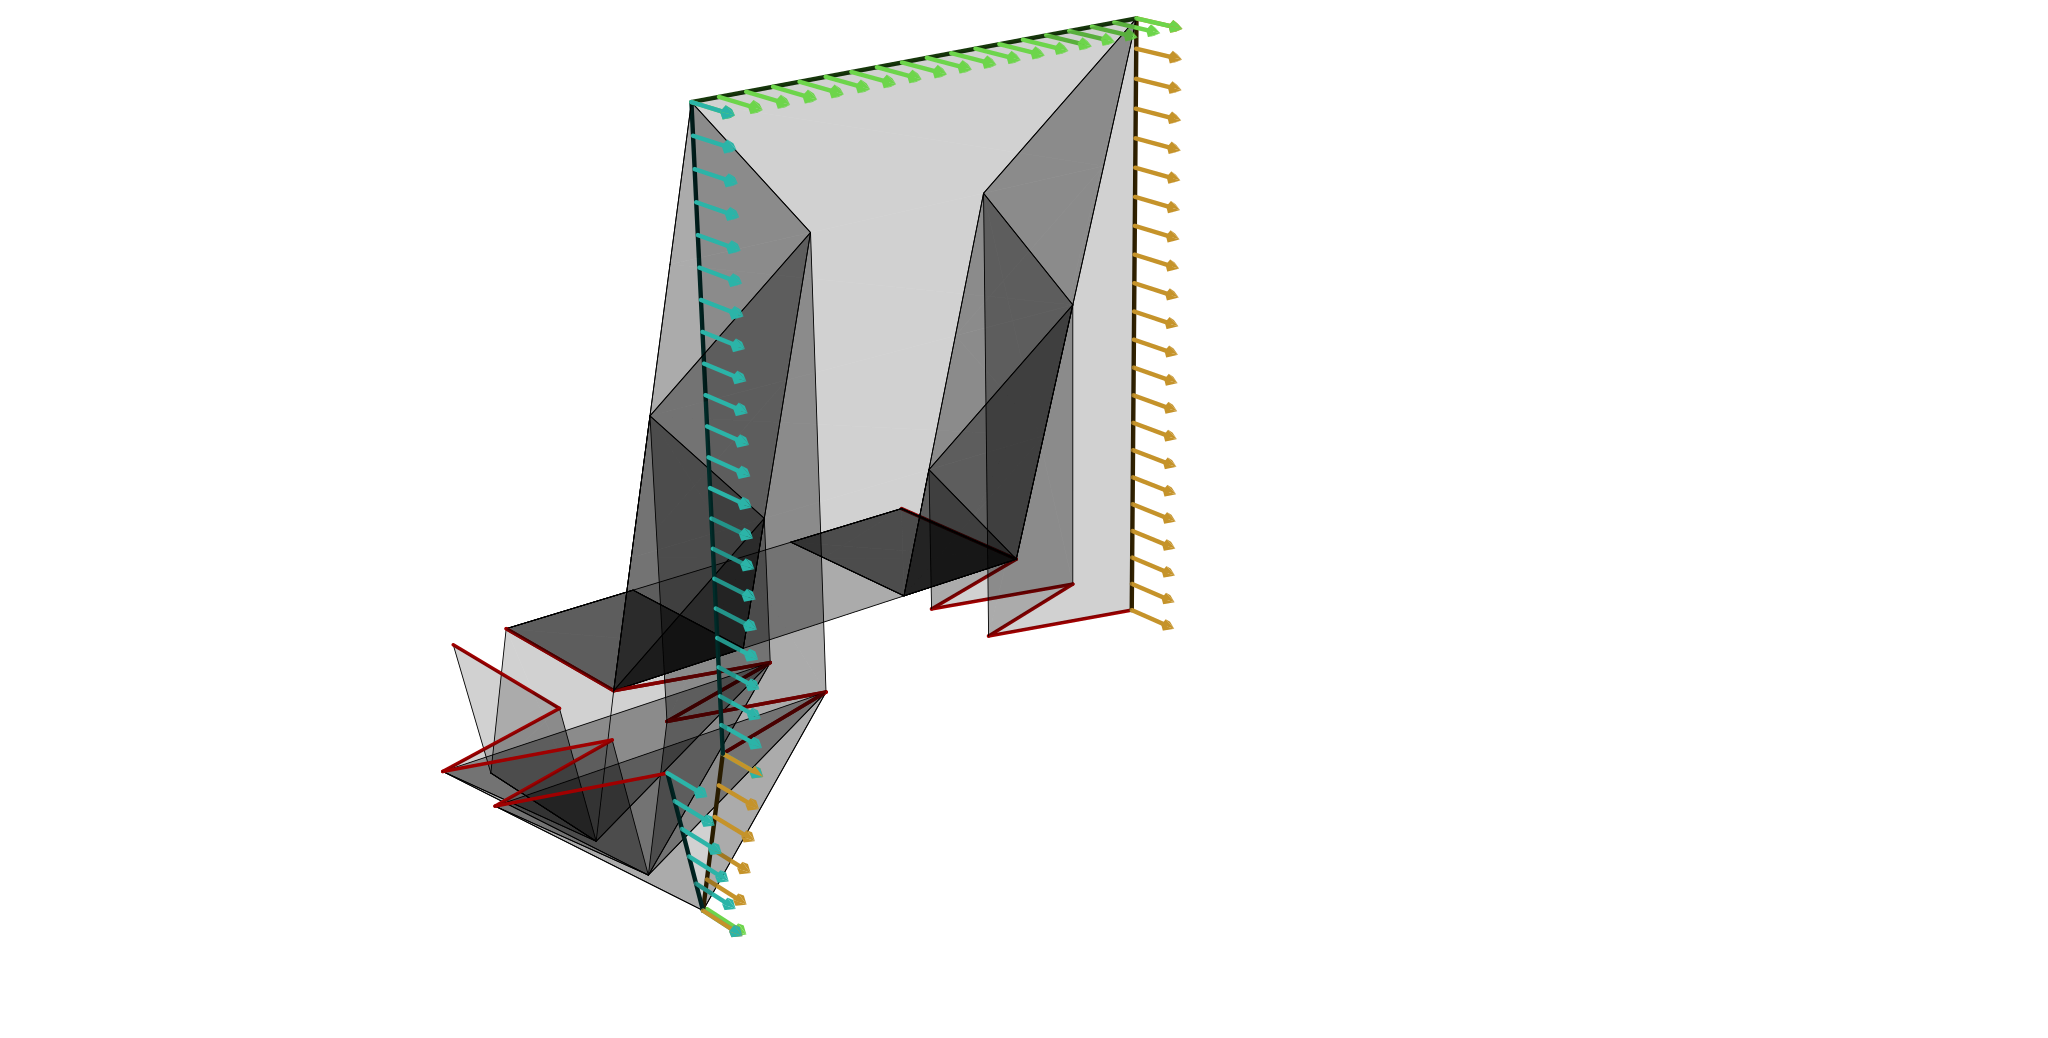
\includegraphics[width=0.35\textwidth]{../figures/column_connector/column10.pdf}%
        \label{fig:column_connector}
    }%
    \caption{}
    \label{fig:connector}
\end{figure}


\end{document}
